\let\negmedspace\undefined
\let\negthickspace\undefined
\documentclass[journal]{IEEEtran}
\usepackage[a5paper, margin=10mm, onecolumn]{geometry}
\usepackage{tfrupee}

\setlength{\headheight}{1cm}
\setlength{\headsep}{0mm}

\usepackage{gvv-book}
\usepackage{gvv}
\usepackage{cite}
\usepackage{amsmath,amssymb,amsfonts,amsthm}
\usepackage{algorithmic}
\usepackage{graphicx}
\usepackage{textcomp}
\usepackage{xcolor}
\usepackage{txfonts}
\usepackage{listings}
\usepackage{enumitem}
\usepackage{mathtools}
\usepackage{gensymb}
\usepackage{comment}
\usepackage[breaklinks=true]{hyperref}
\usepackage{tkz-euclide} 
\usepackage{listings}

\graphicspath{{./figs/}}

\begin{document}
\title{1.11.12}
\author{AI25BTECH11010 - Dhanush Kumar}
\maketitle
\renewcommand{\thefigure}{\theenumi}
\renewcommand{\thetable}{\theenumi}

\noindent
\noindent\textbf{Question:} 

If the sum of two unit vectors is a unit vector, prove that the magnitude of their difference is $\sqrt{3}$.

\bigskip
\noindent\textbf{Solution:} \\


Let 
	$\vec{u}$ and $\vec{v}$ be unit vectors.\\
	Hence,
\begin{align}
	\vec{u}^T \vec{u} &= 1, & \vec{v}^T \vec{v} &= 1.
\end{align}

\medskip

\begin{align}
||\vec{u}+\vec{v}||^2 &= (\vec{u}+\vec{v})^T(\vec{u}+\vec{v}) \\
&= \vec{u}^T\vec{u} + \vec{v}^T\vec{v} + 2\vec{u}^T\vec{v} \\
1^2 &= 1 + 1 + 2\vec{u}^T\vec{v} \\
1 &= 2 + 2\vec{u}^T\vec{v} \\
\Rightarrow \quad \vec{u}^T\vec{v} &= -\tfrac{1}{2}.
\end{align}

\medskip

Now,  
\begin{align}
||\vec{u}-\vec{v}||^2 &= (\vec{u}-\vec{v})^T(\vec{u}-\vec{v}) \\
&= \vec{u}^T\vec{u} + \vec{v}^T\vec{v} - 2\vec{u}^T\vec{v} \\
&= 1 + 1 - 2\left(-\tfrac{1}{2}\right) \\
&= 2 + 1 = 3.
\end{align}

Therefore,  
\begin{align}
||\vec{u}-\vec{v}|| = \sqrt{3}.
\end{align}
\noindent\(\therefore\) The required result is proved.
\begin{figure}[H]
  \centering
   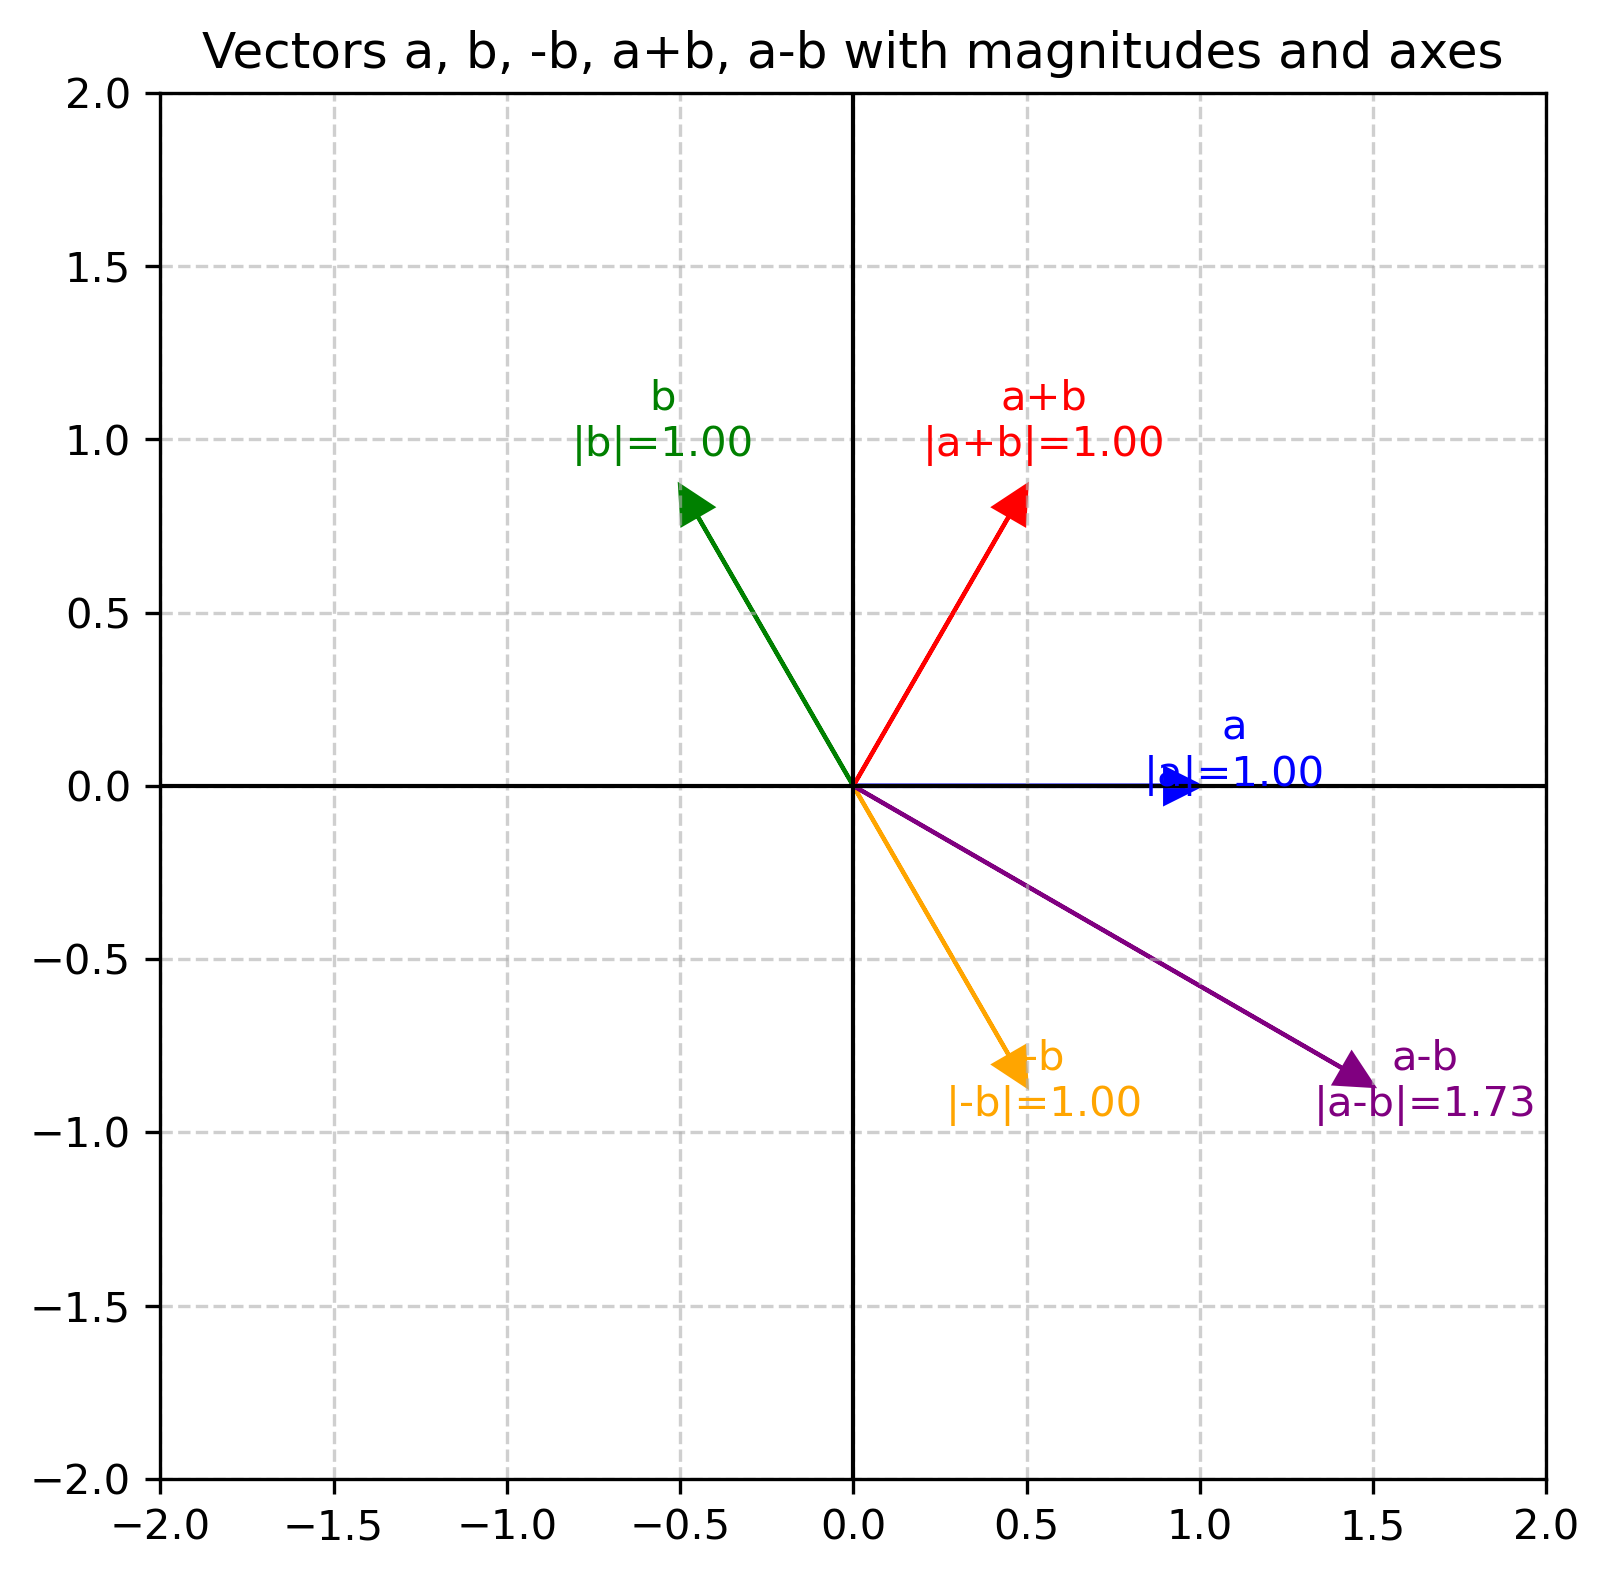
\includegraphics[width=0.7\linewidth]{../figs/vectors_plot.png}
   \caption{}
  \label{stemplot}
\end{figure}


\end{document}

